% TÜ Arvutiteaduse instituudi lõputöö eeskuju ver.2.0
% Tõnu Tamme, 2011
% Jüri Kiho, 2003
% todo: joonised, leheküljemõõdud, numbripunktid, mac, lyx
% iconv -f ISO_8859-15 -t UTF-8 -o eeskuju_utf8.tex eeskuju.tex
  %preambula ---------------------------------------------------
  \documentclass [12pt,a4paper]{report}
  \newif\ifutf
  \utftrue %lülitab UTF-8 sisse/välja (\utftrue|\utffalse)
  \usepackage[T1]{fontenc} %täpitäht ühe sümbolina
  \ifutf
  \usepackage[utf8]{inputenc} %sisendfaili koodilehekylg UTF-8
  \usepackage{ut_thesis_utf8}% ver.0.6
  \else
  \usepackage[latin1]{inputenc} %sisendfaili koodilehekylg ISO 8859-1
  \usepackage{ut_thesis}% ver.0.6  
  \fi
  \usepackage[english]{babel}
  %\usepackage{times} %Times New Roman
  \usepackage{indentfirst} %esimene lõik taandega
  \usepackage{graphicx} %joonised failidena
  \usepackage{algorithm2e}
  \usepackage{multirow}
%  \usepackage{pdfcomment}
  \newcommand{\pdfcomment}[1]{}
  \newcommand{\comment}[1]{}
%\usepackage[margin=1in]{geometry}
%\usepackage[showframe]{geometry}
  %\usepackage{url} %\url
  \usepackage{hyperref} %\url+lingid
  \renewcommand\url{\begingroup\urlstyle{rm}\Url} 
  \usepackage{amssymb,amsmath,amsthm}
  \renewcommand{\leq}{\leqslant} %väiksem-või-võrdne märk eriti ilusasti
  \renewcommand{\geq}{\geqslant} %suurem-või-võrdne märk eriti ilusasti
\newcommand{\TM}{$^{\mathrm{tm}}$ }
  \sloppy
  % ------------------------------------------------------------

%\documentclass{report}
%\usepackage{hyperref}
\usepackage{cite}
%\author{Karl Potisepp, Pelle Jakovits, Satish Narayana Srirama}
%\date{\today}
%\title{Large-scale image processing using MapReduce}

\begin{document}

\begin{tiitelleht}
\pealkiri{Large-scale image processing using MapReduce}
\paber{M.Sc. Thesis (30 ECTS)}
\autor{Karl Potisepp}

\teaduskond{Faculty of Mathematics and Computer Science}
\instituut{Institute of Computer Science}
\eriala{Computer Science}

\juhendaja{Pelle Jakovits M.Sc., Satish Narayana Srirama Ph.D.}

\end{tiitelleht}

%\maketitle

\tableofcontents

\chapter{Introduction}

Along with the development of information technology, a constant stream of new applications for solving humanity's problems has also appeared. As we possess more computing power, we can tackle more and more resource-intensive problems such as DNA sequencing, seismic imaging and weather simulations. When looking at these subjects, a common theme emerges: all of these involve either analysis or generation of large amounts of data. While personal computers have gone through a staggering increase in power during the last 20 years, and the processing power even within everyday accessories - such as smartphones - is very capable of solving problems that were unfeasible for supercomputers only a couple of decades ago, analysing the amount of data generated by newest generation scientific equipment is still out of reach in some areas. Moreover, as processor architectures are reaching their physical limitations with regard to how small individual logic gates and components can get, using distributed computing technologies has become a popular way to solve problems which do not fit the confines of a single computer. Supercomputers, GRID-based systems and computing clouds are an example of this approach. Since the fields of distributed computing and image processing are too broad to fully cover in this thesis, this work will focus on the latter of the three with regard to image processing.

Due to the increasing popularity of personal computers, smart televisions, smartphones, tablets and other devices carrying a full-fledged operating system such as Android, iOS or Windows 8, and due to the capability of these devices to act as producers of many kinds of content instead of being passive receivers (like radio and television, for example), there is a need to be able to process that content. Photos need to be resized, cropped and cleaned up, and recorded sound and video need to be shaped into a coherent whole with the aid of editing software. These procedures however may not be something that is best tackled on the same device that was used for recording, because of limiting factors in processing power, storage space and - in some cases - battery life. However with the widespread availability of wireless internet or high-throughput cell phone networks, any of the aforementioned devices can simply upload their data to a more capable computer in order to do necessary processing. 

As in many cases the recorded media will be consumed using a different device (for example, viewing holiday photos taken with your smartphone on your computer or smart TV), it can be argued that both the steps of transferring media from the recording device and processing it are inevitable anyway. Facebook and YouTube both provide a good example of this scenario: the user can upload their media in more or less in an unprocessed format and the frameworks take care of resizing and re-encoding the media so that it can be consumed by users. However, since these services are very popular, as a consequence the amounts of data that is needed to process are also huge. For example, 72 hours of video data is uploaded to YouTube every minute \cite{youtube_stats}. Even without going into details of video compression or the processing pipelines involved, it is easy to see how even a day's worth of uploads (103 680 hours) quickly becomes unfeasible to compute without resorting to distributed computing.

For solving processing tasks involving data of this scale, engineers at Google (the parent company of YouTube) designed the MapReduce model of distributed computing, of which Apache Hadoop is the most popular open source implementation. It is well known that using the MapReduce model is a good solution for many problems, however judging from the work done in the field of distributed computing with regard to image processing, the suitability of the model for this application not very well known. In this thesis I will describe the MapReduce model, it's implementation in the form of Hadoop, and explore the feasibility of using this technology for doing large scale image processing.

The rest of this work is structured as follows. In the next sections I will describe in more detail the terminology and the problem at hand, give a brief overview of previous work in this area. Chapter 2 will focus on describing the MapReduce model and the specifics of it's implementation in Apache Hadoop. In chapter 4 I will look at two different practical use cases for applying MapReduce to large scale image data. The fifth and final chapter provides an overview of the results and outputs of this thesis. TODO obviously rewrite this part after the structure finalised. %TODO

%Image processing, high resolution medical images, cheap quality cameras and abundance of photos. Also cheap hard drives which allow to store all this stuff. TODO explain :)

%In this thesis, I will describe solving two different image processing tasks related to two-dimensional colour images using the Hadoop open source distributed computing framework. %TODO

%Description in broad terms of what has been achieved with this thesis.

%Possible subtopics:
%\begin{itemize}
%	\item Microscope photo processing with bilateral filter - Datexim SAS (ENSICAEN)
%	\item de-noising satellite images (maybe)
%	\item Classification and metadata extraction from archaeological excavation data (TO BE ELABORATED)- Graeme Earl and Hembo Pagi (U of Southampton)
	
%\end{itemize}

\section{Problem statement}

Before going deeper into details, I will first specify the size of data I consider to be large-scale with with regard to this work. This requires some grossly simplified description of the architecture of shared amongst all modern computers. It is common knowledge that a computer consists of a processor, memory and a hard drive. The processor performs calculations on the data stored in memory, which has previously been read from a hard drive. It is important to note here that since very many computers are also connected to the Internet, the hard drive in question may reside in a different physical location than the processing unit and memory. Now, it is also known that the data transfer speed between the processor and memory is generally orders of magnitude faster than between memory and hard drive. Similarly, reading from a local hard drive is faster than accessing data from storage in a different computer, due to overhead added by having to communicate over a network.

Therefore, as the size of the data to be processed by one algorithm increases so that the computer no longer can hold all the information in memory, there is a significant decrease in processing speed. Similarly, if the data does not fit on the local hard drive, the processing speed drops due to having to wait for it to be sent in from another computer. While this can be alleviated somewhat by using buffering techniques, the general rule remains the same: it's best if the problem fits within memory, worse if it fits on the local hard drive and worst if the data has to be read across the network. Processing a large image is an example of such a problem.

In this case we are dealing with a microscope image with a resolution of 86273 by 81025 pixels (roughly 6.99 gigapixels), where each pixel is made up of 3 values - red, green and blue. Assuming that each of these values is stored as a 32-bit precision floating point number, the total memory consumption of storing this data in an uncompressed way can easily be calculated:

\begin{center}
$ 86273 * 81025 * 3 * 32$ bits $ = 78.12 $ gigabytes.
\end{center}

At the time of writing this document, most commodity computers do not have the required memory to even store this amount of data, and certainly not to perform any sort of processing with an overhead dependent on the input size, and even though there do exist specialised computers with enough memory for solving this issue, they are significantly more expensive to acquire and maintain. However, our aim is to find out whether it is possible  to process this kind of images using commodity computers in such a way that all the necessary data is stored within memory.

The second case involves a data set of 48469 images totalling 308 GiB (the average image here is a JPEG2000 file around 6.5MiB in size). While the size of the data set is small enough to fit on regular hard drives, and processing the images individually is not a problem, because the average size remains around 13 megapixels, thus requiring roughly only 40 MiB of memory, which is orders of magnitude less than was the case with the large image. In this case, the issue is not so much being able to fit the problem within memory, but rather about being able to process the data quickly enough. Here we depend on the processor - it does not matter how many more images you can fit inside the memory since generally the processor can only work on one image at a time. In reality, this depends on how many cores the processor has and how well the algorithm can take advantage of that, but even with many cores, going through all of the data can be very time-consuming. Therefore, the problem to solve in this case is how to process this data set in an efficient way.

In this section I have established that processing the aforementioned classes of large images or large data sets of regular images can not be done on a single personal computer, because in the first case, they do not fit into memory, and in the second case one computer can not process them fast enough. Neither of these issues can be expected to be solved by advances in computing power, because CPUs are already reaching their theoretical physical limitations  and the scale of data is increasing faster than the processing capabilities of single commodity computers. 

A solution for these problems is turning towards distributed computing, where limitations of a single computer are overcome by combining the resources of many computers to perform one large task. While this approach is not new - supercomputers and computing clusters have existed for many years already - it is only recently that techniques of using commodity computers for distributed processing have gained popularity. In the following I will explain more thoroughly how these technologies could be used to solve image processing tasks.

\subsection{Distributed image processing}

Since this thesis is focused on using the MapReduce model for performing image processing, I will now describe some of the issues that stem from the limitations of this model with regard to images. I will also restrict the problem space to 2-dimensional colour images. This may not seem like much of a change at first, as it is probably the most common definition for an image, yet it allows us to disregard issues related to videos, 3-dimensional meshes and other types of image data that is also studied in the field of image processing. Finally, I will further divide image processing problems into four classes: iterative local and non-local algorithms and non-iterative local and non-local algorithms.

Generally speaking, the MapReduce parallel computing model follows what can be called a divide-and-conquer strategy of parallelised computing. That is, instead of joining together physical resources like processing power, memory and hard drive storage in order to allow the processing software to see these combined devices as one monolithic entity, the problem is divided into independent parts which are then processed separately - usually in different physical or virtual computers - and later joined together to form the output. In the following I will explain how this affects the parallelisation of image processing algorithms.

Local, with regard to image processing, denotes that the computation is performed as a series of small calculations on fixed subsets of the image: typically this means that the value of a pixel in focus is re-calculated using the values of it's neighbouring pixels. It is easy to see how problems like this can be parallelised by virtue of splitting the image into parts, performing the processing, and later putting it back together. Gaussian blurring, which I will briefly describe during the course of this work, is an example of a local processing algorithm. Contrary to local, non-local problems involve larger parts of the image. A good example of non-local processing is object recognition. For example, in order for a trained character recognition algorithm to be able to recognise the letter "A" from an image, it's search window needs to be big enough to encompass the whole letter (see figure \ref{fig_local_nonlocal}). The solution of splitting the image into parts to allow for parallel processing now requires special attention in order to avoid splitting objects into unrecognisable fragments, and in the worst case could be entirely inapplicable if the object to be classified takes up the whole image.

\begin{figure}[h]
\begin{center}
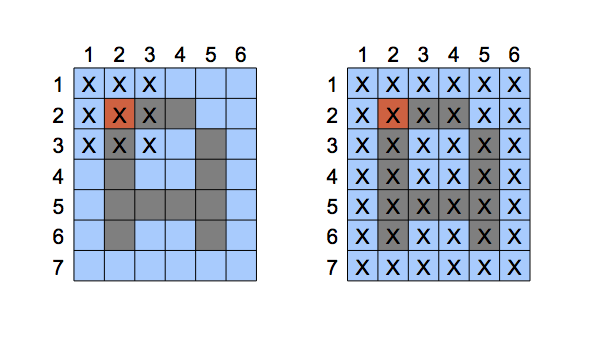
\includegraphics[]{local_nonlocal.eps} %TODO render with PDF
%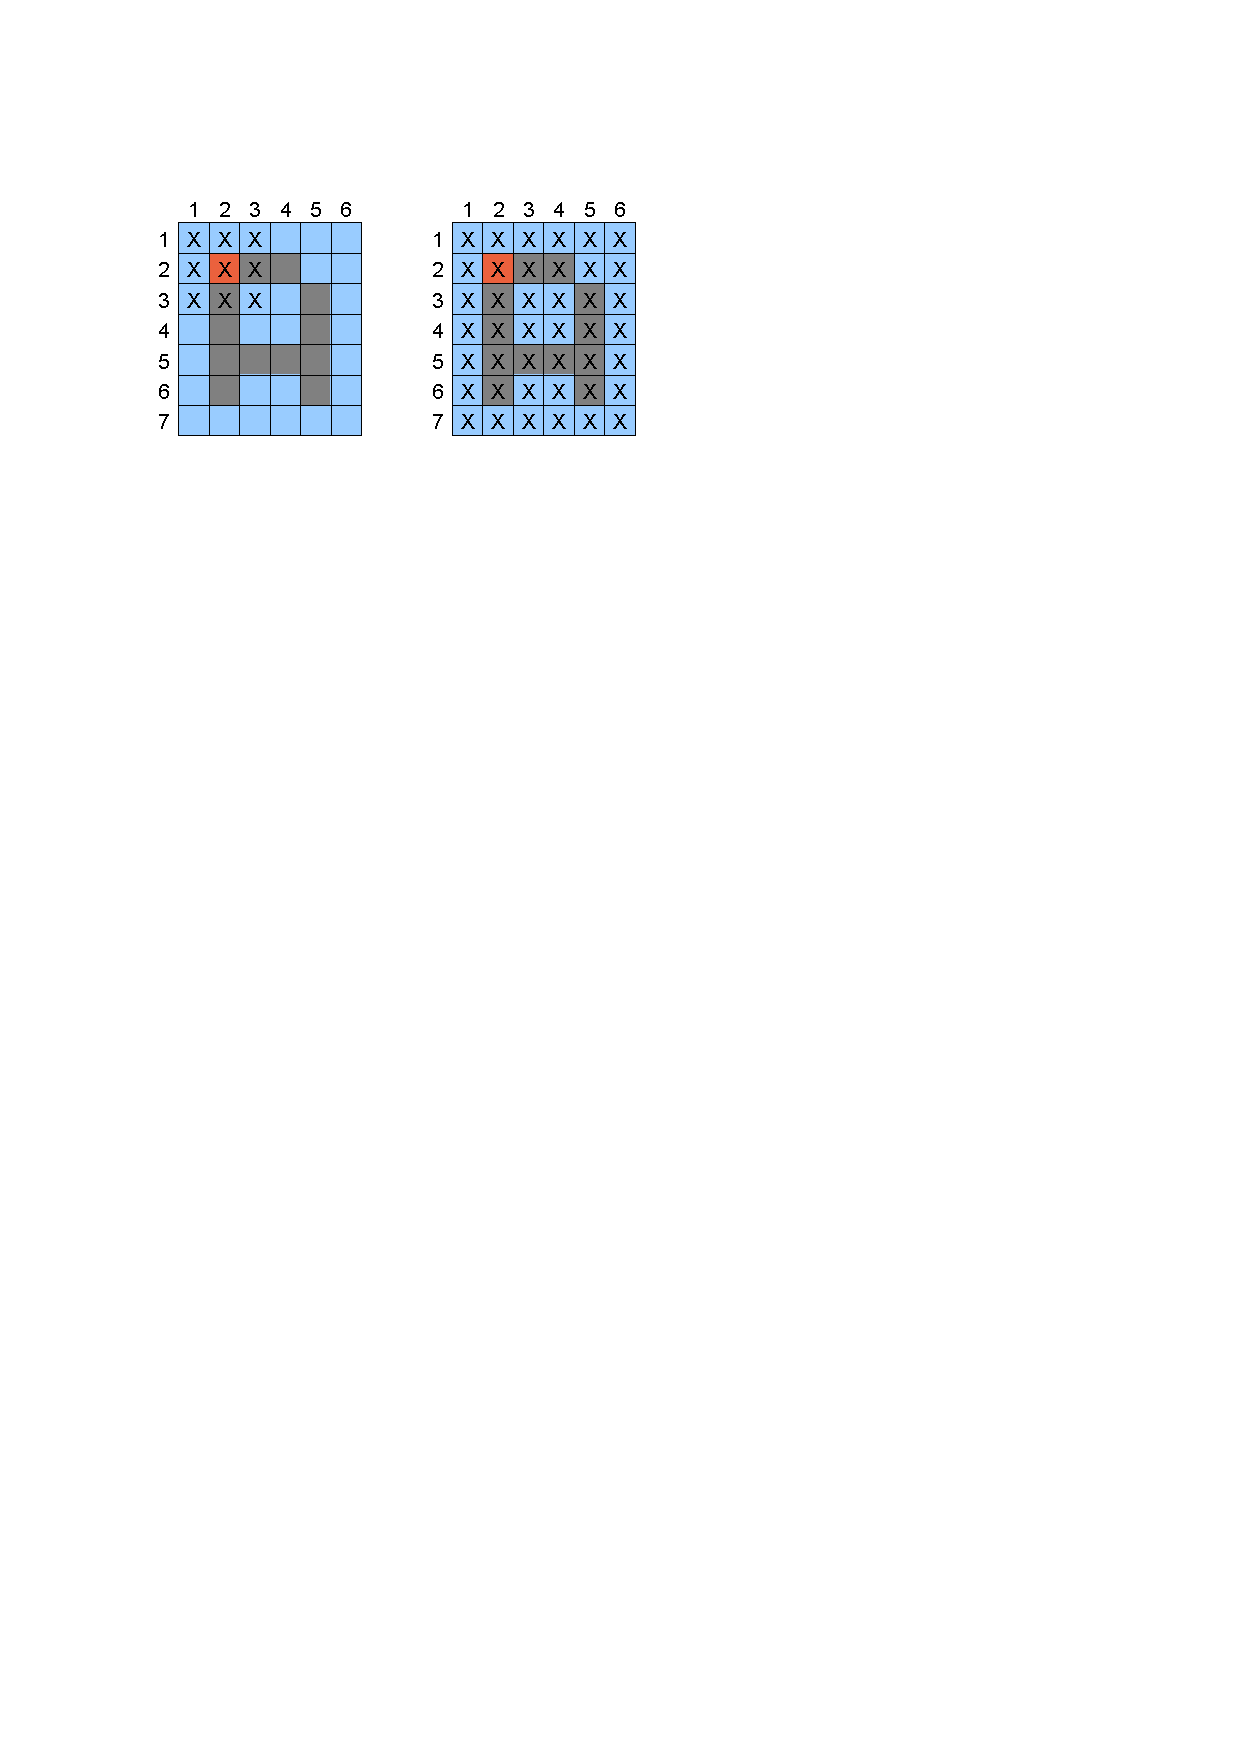
\includegraphics[]{local_nonlocal.pdf} %render with PDF
\caption{Differences between local (left) and non-local (right) processing. Red represents the pixel in focus, the X-s represent the pixels whose data the algorithm needs to access.}
\label{fig_local_nonlocal}
\end{center}
\end{figure}

The distinction between iterative and non-iterative algorithms is simpler: a non-iterative algorithm only processes the image a constant number of times - depending on the algorithm, up to five or six - to achieve the desired effect, whereas an iterative algorithm requires multiple passes, and often the output image of a previous pass becomes the input of the next pass. Observing the data requirements for what simply seems an iterative local algorithm, it is easy to see that even though the resulting values for pixels in the first pass only depend on their close neighborhood, from the second iteration on, those adjacent pixels have had their values adjusted according to their neighborhoods, which in turn are changed according to their neighbors and so on (see figure \ref{fig_local_iterative}). While the extent of this influence depends on the algorithm in question, the algorithm itself is - strictly speaking - non-local.

\begin{figure}[h]
\begin{center}
\includegraphics[scale=0.8]{local_iterative.eps} %TODO render with PDF
%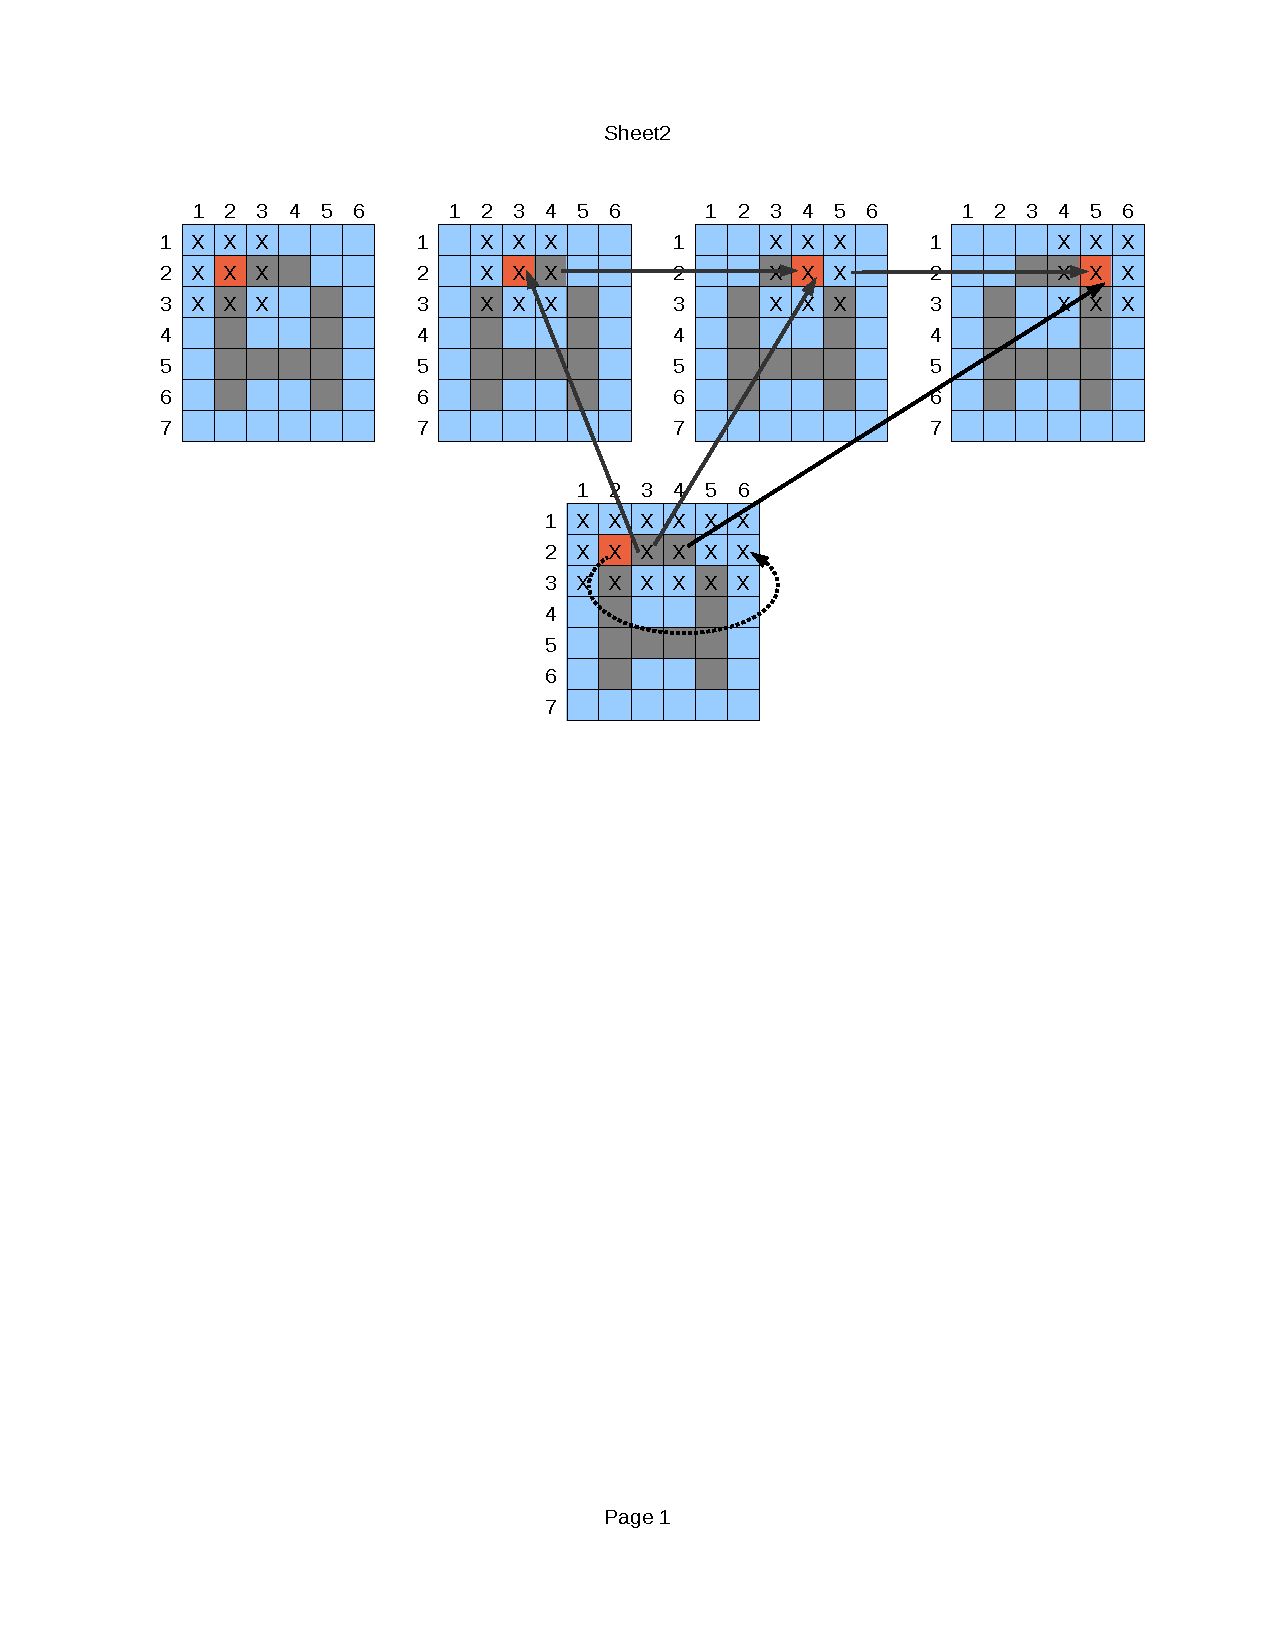
\includegraphics[scale=0.8]{local_iterative.pdf} %render with PDF
\caption{Illustration of the data requirements of iterative local processing. The top row represents first local computations of the first iteration. The diagram on the bottom shows the requirements at the start of the second iteration. Arrows encode a 'depends on' relationship: the value from which the arrow originates depends on the value the arrow is pointing at.}
\label{fig_local_iterative}
\end{center}
\end{figure}

Therefore, we can establish four classes of image processing problems: local, non-local, iterative local and iterative non-local. We can now look back at the example cases brought up previously and see what issues would arise if we attempted to parallelise local and non-local algorithms on these images.

In the first case, it immediately becomes obvious that parallelising a non-local type of algorithm is going to be a non-trivial task, as we lack even the ability to store it in memory. Even when assuming that the algorithm can continue to function if the input image is split to pieces, if communication is also required between the computers working on separate pieces, then there is a good chance that network speed will become a bottleneck and slow down the computation.

The second case, however, is far more suited for processing with the MapReduce model. Even though the total size of the data several times bigger than in the first case, since it consists of comparatively small images which easily fit into memory even when taking any algorithm-specific overhead into account. Moreover, because we do not have to split any images into pieces or worry about communication between worker computers, classification of the algorithms into the aforementioned four groups does not matter. Therefore, looking at the issues with regard to analysing this sort of data lets us make conclusions that apply to a wider range of problems. 

At this point it is important to note that we have so far silently assumed that all the algorithms we classify only require one image as an input. Speaking from the perspective of distributed processing, this means we assume that the algorithm only requires data from one image at a time. For example, with this clause we exclude any processing that needs to compare two or more images with each other from this discussion. The reason behind this will become clear further on in this text, as it is somewhat related to the implementation of the MapReduce model in Apache Hadoop and our approach to parallelising image processing tasks by dividing images into manageable pieces. Briefly and informally, it can be summarised as follows: if an algorithm requires access to more images than the local storage of the computer allows, communication between computers is needed. However, since a MapReduce calculation has only one step where the computing nodes exchange information, the only way to satisfy this need without resorting to another processing model is to run the MapReduce calculations themselves iteratively (note that when speaking about iterative image processing algorithms, I mean that all the iterations will be done within one MapReduce calculation). This, in turn, has been shown by Satish Srirama et al. to be very slow in actual performance, especially as the number of iterations increases \cite{srirama2012adapting}.

\subsection{Why use MapReduce?}

In the previous sections, I have presented some general analysis with regard to the general feasibility of using the MapReduce model of distributed computing to solve image processing tasks. In this part I will summarise the main motivation behind choosing MapReduce and it's implementation in the form of Apache Hadoop, and briefly outline alternative ways how one could approach distributed image processing.

First, what are the alternatives? Batch processing on the PC is feasible for only small amounts of data, and since only a part of this data fits into memory at given time, computation will suffer from a decrease in speed due to slow hard drive access. Trying to counter this by running the batch process on several computers simultaneously is a solution, but it creates a need for job monitoring, mechanisms for data distribution and means to ensure that the processing completes even when some computers experience failures during work. This is more or less exactly the problem that both Google MapReduce and Apache Hadoop were designed to solve. Another approach is treating the problem like a traditional large-scale computing task which requires specialised hardware and complex parallel programming. Cluster computers built on graphics processing units (GPU) are an example of this, and while maintaining a purpose-built computer cluster has been shown to be a working solution for many kinds of problems, it is interesting to know whether the same issues can be tackled with simpler and cheaper systems without much decrease in efficiency.

In conclusion, the main motivation behind using MapReduce (and more specifically Apache Hadoop) for image processing can be summed up in the following: as performing image processing is something that has already become a popular application of computing technology for an increasing amount of people, and because these tasks often require more processing capability than ordinary computers have, there is a need to turn towards distributed computing. On the other hand, since the MapReduce model implemented by Hadoop is currently one of the more popular such frameworks, it is a logical choice for trying to solve these processing issues, as it is freely available, provides a reliable platform for parallelising computation and does not have any requirements with regard to specialised hardware or software.

\chapter{Background}

In this chapter I will describe and summarise relevant work that has been done in the field of distributed image processing, then describe the MapReduce computing model with regard to Apache Hadoop and Hadoop Distributed Filesystem.

\section{Relevant work}

In order to gauge the relevance of addressing the problems brought up in the previous chapter, I will provide in the following text a brief overview of previous work sharing the themes of image processing and distributed computing in no particular order. 

In Web-Scale Computer Vision using MapReduce for Multimedia Data Mining \cite{White:2010:WCV:1814245.1814254}, Brandyn White et al. present a case study of classifying and clustering billions of regular images using MapReduce. No mention is made of average image dimensions or any issues with not being able to process certain images because of memory limitations. However, a way of pre-processing images for use in a sliding-window approach for object recognition is described. Therefore one can assume that in this approach, the size of images is not an issue, because the pre-processing phase cuts everything into a manageable size. The question still remains whether a sliding window approach is capable of recognizing any objects present in the image that do not easily fit into one analysis window, and whether the resource requirements for image classification and image processing are significantly different or not.

An Architecture for Distributed High Performance Video Processing in the Cloud \cite{Pereira:2010:ADH:1844768.1845374} by Rafael Pereira et al. outlines some of the limitations of the MapReduce model when dealing with high-speed video encoding, namely it's dependence on the NameNode as a single point of failure (however a fix is claimed at \cite{website:facebook_namenode_improvements}), and lack of possibility for generalization in order to suit the issue at hand. An alternative - optimized - implementation is proposed for providing a cloud-based IaaS (Infrastructure as a Service) solution. However, considering the advances of distributed computation technology within the past two years (the article was published in 2010) and the fact that the processing of large images was not touched upon, the problem posed in this work still remains.

A description of a MapReduce-based approach for nearest-neighbor clustering by Liu Ting et al. is presented in Clustering Billions of Images with Large Scale Nearest Neighbor Search \cite{citeulike:2631015}. This report focuses more on the technicalities of adapting a spill-tree based approach for use on multiple machines. Also, a way for compressing image information into smaller feature vectors is described. With regards to this thesis, again the focus is not so much on processing the images to attain some other result than something intermediate to be used in search and clustering.

In Parallel K-Means Clustering of Remote Sensing Images Based on MapReduce \cite{Lv:2010:PKC:1927661.1927687}, Lv Zhenhua et al. describe using the k-means algorithm in conjunction with MapReduce and satellite/aerophoto images in order to find different elements based on their color (i.e. separate trees from buildings). Not much is told about encountering and overcoming the issues of analyzing large images besides mentioning that a non-parallel approach was unable to process images larger than 1000x1000 pixels, and that the use of a MapReduce-based parallel processor required the conversion of TIFF files into a plaintext format.

Case Study of Scientific Data Processing on a Cloud Using Hadoop \cite{Zhang:2009:CSS:2127968.2128002} from Zhang Chen et al. describes the methods used for processing sequences of microscope images of live cells. The images and data in question are relatively small - 512x512 16-bit pixels, stored in folders measuring 90MB - there were some issues with regard to fitting into Hadoop DFS blocks which were solved by implementing custom InputFormat, InputSplit and RecordReader classes. No mention was made about the algorithm used to extract data from the images besides that it was written in MATLAB and MapReduce was only involved as a means distribute data and start the MATLAB scripts for processing.

Using Transaction Based Parallel Computing to Solve Image Processing and Computational Physics Problems \cite{trease08} by Harold Trease et al. describes the use of distributed computing with two examples - video processing/analysis and subsurface transport. The main focus is put on the specifications of the technology used (Apache Hadoop, PNNL MeDICI), whereas there is no information presented on how the image processing parts of the examples given were implemented.

In Distributed frameworks and parallel algorithms for processing large-scale geographic data \cite{Hawick:2003:DFP:958021.958024}, Kenneth Hawik et al. describe many problems and solutions with regard to processing large sets of geographic information systems' (commonly known as GIS) data in order to enable knowledge extraction. This article was published in 2003, so while some of the issues have disappeared due to the increase in computing power available to scientists, problems stemming from the ever-increasing amount of data generated by different types of monitoring technologies (such as ensuring distribution of data to computation nodes and storing big chunks of data in memory) still remain. Also, considering that the Amazon EC2 \cite{website:amazon_ec2} web service came online just in 2006, it is obvious that one can not make an apt comparison whether or not a MapReduce-based solution in 2012 is better or not for large-scale image processing than what was possible using grid technology in 2003.

A Scalable Image Processing Framework for gigapixel Mars and other celestial body  images \cite{5446706} by Mark Powell et al. describes the way NASA handles processing of celestial images captured by the Mars orbiter and rovers. Clear and concise descriptions are provided for the segmentation of gigapixel images into tiles, how these tiles are processed, and how the image processing framework handles scaling and works with distributed processing. The authors used the Kakadu JPEG2000 encoder and decoder along with the Kakadu Java Native Interface to develop their own processing suite. The software is proprietary and requires the purchase of a license to use.

Ultra-fast processing of gigapixel Tissue MicroArray images using high performance computing \cite{wang2011ult} by Yinhai Wang et al. talks about speeding up the analysis of Tissue MicroArray images by substituting human expert analysis for automated processing algorithms. While the images sizes processed were measured in gigapixels, the content of the image (scans of tissue microarrays) was easily segmented and there was no need to focus on being able to analyse all of the image at once. Furthermore, the work was all done on a specially built grid high performance computing platform with shared memory and storage, whereas this thesis is focused on performing processing on a Apache Hadoop cluster.

While the above shows that there has been a lot of work in this area the question remains whether (and how well) Hadoop is suited for large scale image processing tasks, because as evidenced by this brief overview, there are only a few cases where image processing has been done with MapReduce. 

%In this chapter I will provide a thorough description of all technologies and methodologies that are important with regards to this work. I will describe the operating philosophy of the MapReduce model and the capabilities and limitations of it's most popular freely non-proprietary implementation - Hadoop. Also, the different image processing and Java-C++ technologies used while working on this thesis, such as the CImg library and the Java Native Interface, will be elaborated.

\section{MapReduce}

MapReduce is a programming model developed by Google for processing and generating large datasets used in practice for many real-world tasks \cite{Dean:2008:MSD:1327452.1327492}. In this section, I will focus on describing the general philosophy and methodology behind this model, whereas the following part will describe in more detail one of the more popular implementations of the model - Hadoop - which is also used for all the practical applications featured in this work.

The basic idea behind MapReduce is based on the observation that a lot of processing tasks involving terabytes of data need to deal with the issues of distributing the data across a network of computers to ensure that the available storage and CPU resources are maximally utilised, and it would be easier if programmers could focus on writing the processing part that is actually different per task. To achieve that end, the developer has to define only two functions - \textit{Map} and \textit{Reduce} - while everything else is already set in place by the model's definition. Actual implementations provide many more functionalities and parameters to tweak in order to help the model to better conform to the task at hand, however this core functionality can not be changed. Essentially, a MapReduce computation can be described as the following series of steps:

\begin{enumerate}
\item Input is read from disk, converted to Key-Value pairs.
\item The \textit{Map} function processes each pair separately, and outputs the result as any number of Key-Value pairs.
\item For each distinct key, the Reduce function processes all Key-Value pairs with that Key, and - similarly to Map - returns any number of Key-Value pairs.
\item Once all input pairs have been processed, the output of the Reduce function is then written to disk as Key-Value pairs. 
\end{enumerate}

At first glance, this mode of computing may seem restrictive. This is true in the sense that when adapting algorithms to this model, radical changes must in some cases be made in order to attain the best possible performance. 

\begin{figure}[h]
\begin{center}
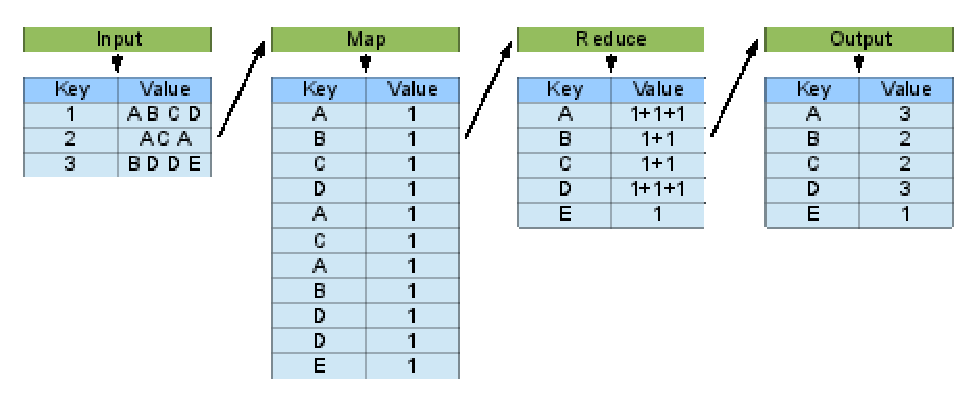
\includegraphics[scale=0.5]{mapreduce.eps} %TODO render with PDF
%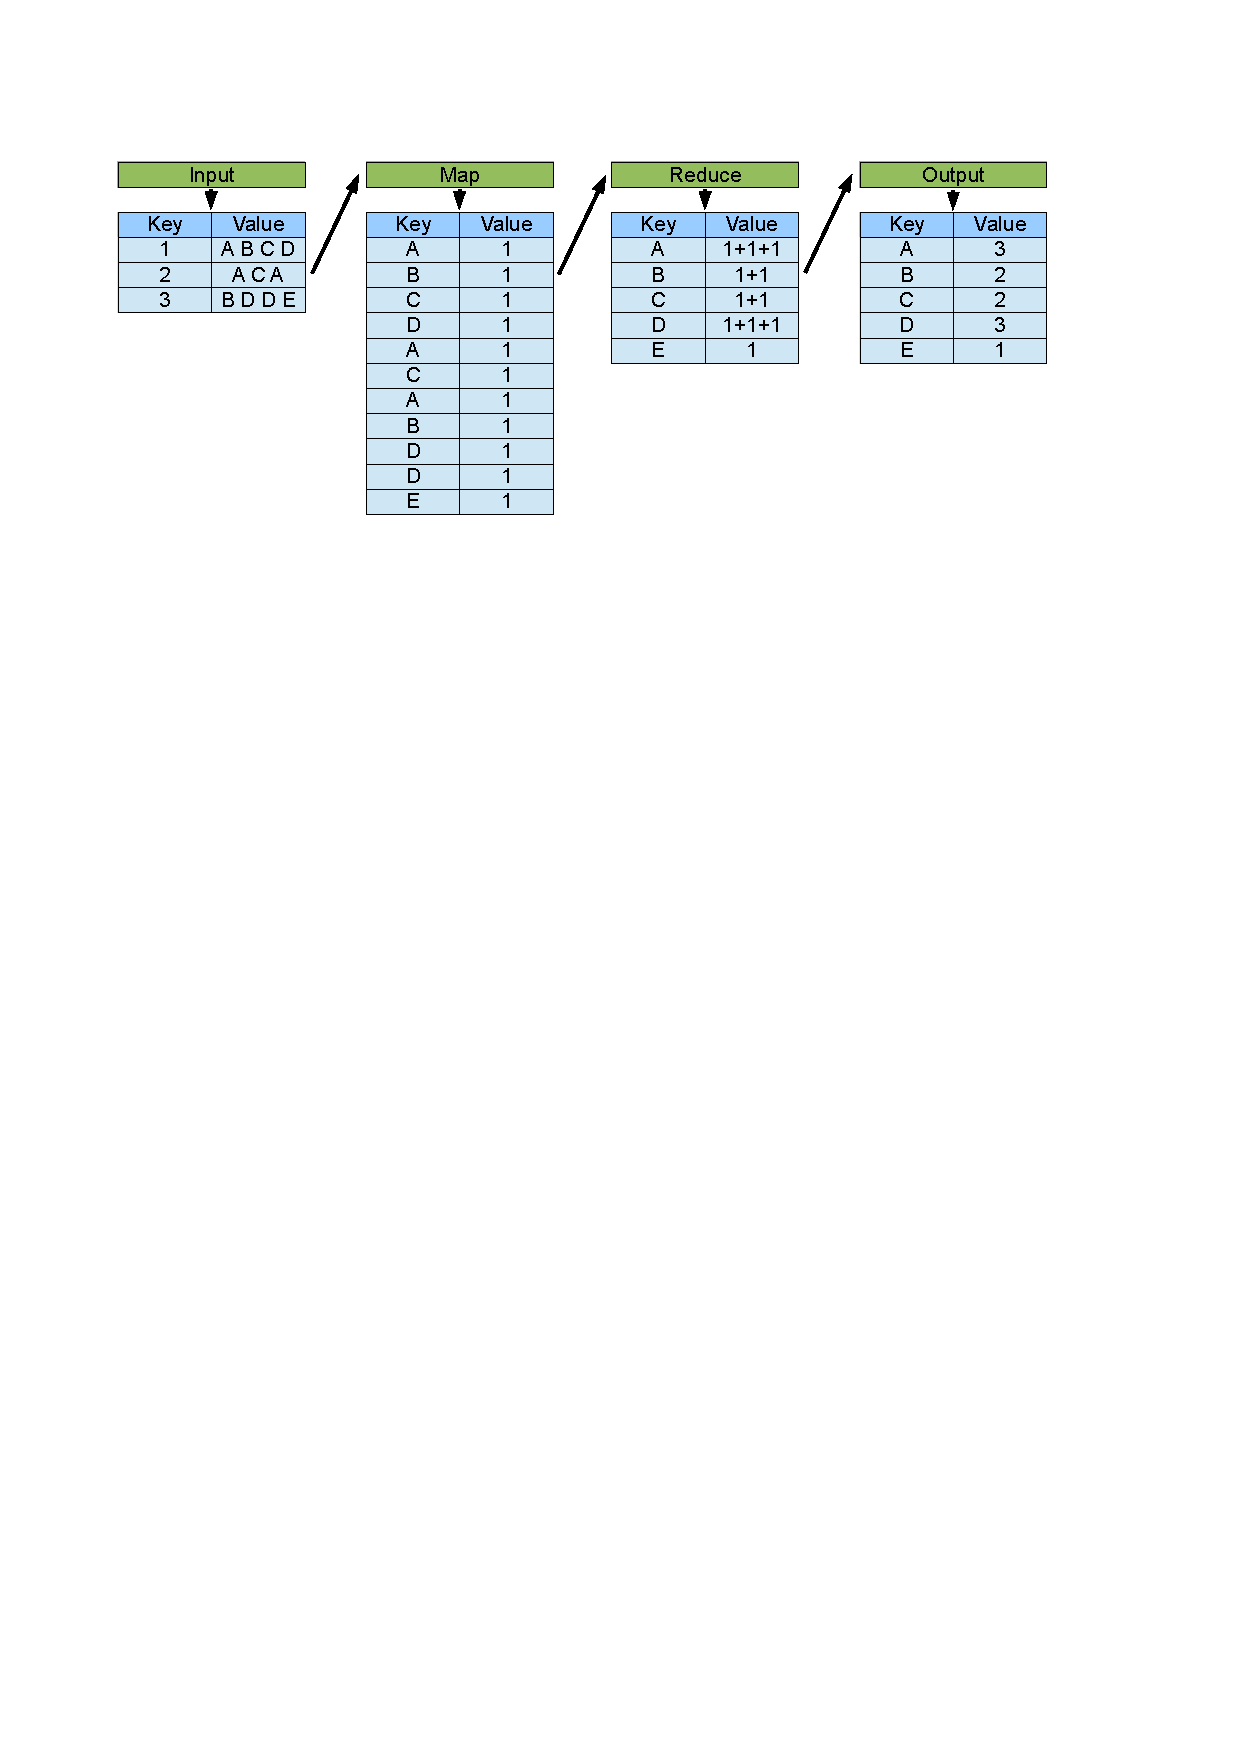
\includegraphics[scale=0.8]{mapreduce.pdf} %render with PDF
\caption{A simple example of the MapReduce computation model, inspired by the WordCount example provided in the Apache Hadoop Getting Started tutorial. A text file is first converted into pairs of line number and its content (Input), then the Map function splits these pairs further so that the reducer receives one pair per occurrence of a word. The objective of the Reduce function is then to count the individual occurrences and finally output the total per each distinct word.}
\label{fig_mapreduce}
\end{center}
\end{figure}
 
%Description of the general philosophy of MapReduce, the logic behind Map/Reduce/etc. parts of the processing chain, and how this approach suits/is cumbersome when dealing with image processing.

\subsection{Apache Hadoop}
Hadoop is an open-source framework for distributed computing developed by the Apache Foundation, inspired by Google's MapReduce (TODO cite Hadoop and MapReduce papers). It has been in development since 2005 and - at the time of writing this work - is one of the most popular freely available applications of it's kind. Due to this and also a large user base ranging from home users to large companies makes Hadoop a good candidate for attempting to use it for image processing.

\subsubsection{Hadoop Distributed File System (HDFS)}
HDFS is the underlying file system that Hadoop uses in order to store data meant to be processed by MapReduce. It is inspired by the Google File System (GFS) (TODO cite). There are two reasons why the file system comes into play when discussing image processing using Hadoop. Firstly, the distributed nature of HDFS ensures that all input data is spread across the cluster's storage so that at least initially every worker can process data stored on it's local hard drive. Secondly, the configured block size somewhat restricts the storage of files - if a file is larger than the block size and can not easily be split, then all it's blocks will have to be stored in the same location, which in essence means that the advantages from having a small block size are lost.
TODO replication, what happens to a file when it is bigger than 1 block size

\subsubsection{Running a MapReduce job}

TODO how to write a job, what to take into account (with regard to images), what are the restrictions w/r/t communication, storage

TODO what is a MapReduce job?

\section{Image processing}

As already mentioned in the preceding text, in this thesis I will restrict my focus with regard to the field of image processing to two-dimensional color images. The following will not be a description of how images are acquired through the use of scanning or digital cameras, therefore it is assumed here that the reader is familiar with the notions of pixels, 2-dimensional coordinate notation and representing color using red, green and blue values. Therefore I will start with the following formal definition: I consider the image $I$ with width $x$ and height $y$ as a collection of pixels $p$, such that

\begin{center}
$I = \{ \, p_{i,j} | \, i \in [1,x], \, j \in [1,y] \, \}$, and

$p_{i,j} = (r_{i,j}, g_{i,j}, b_{i,j})$,
\end{center}
where $r_{i,j}$, $g_{i,j}$ and $b_{i,j}$ are respectively the red, green and blue values of the pixel at $x$-coordinate $i$ and $y$-coordinate $j$. From this definition it is more or less straightforward to estimate the minimal memory requirements for storing an image with known dimensions when the programming language and data type for storing individual color values is also chosen. Since this thesis deals with Java, and image processing algorithms tend to prefer floating point values (which are 32 bits in Java) in the interests of precision, we can estimate the memory consumption $M$ of an image with dimensions $x$ and $y$ as follows:

\begin{center} 
$M = x * y * 3 * 32$ bits.
\end{center}

As image processing algorithms tend to operate on uncompressed images, using this sort of calculations provides a way of estimating the memory requirements from the time complexity of the processing tasks. Therefore the size of compressed the image file (for example JPEG or PNG) is only very loosely correlated with the time it takes to process that image, as the efficiency of compression algorithms depends on the information content of the image itself, whereas the estimation method described above only takes into account the spatial dimensions of the image.

\subsection{Common applications}

TODO gaussian blur, edge detection, etc. with processing requirements

\subsection{ImageJ}
For processing images while working on the practical part of this thesis, I used the ImageJ library. It is a freely available image processing application written in Java and developed by the National Institutes of Health \cite{imagej}. It supports the processing and analysis of a wide variety of image types (8-, 16-, 32-bit RGB/black \& white images) and many commonly used image file formats such as PNG, TIFF and JPEG.

TODO how was imagej used in the work

\subsection{OpenCV}

\subsection{Tesseract}

\subsection{Pandore}

\subsection{ImageMagick}

\section{Image processing and MapReduce}

It is known that the MapReduce method places some restrictions on iterative parallel processing algorithms that require communication between computing nodes. Since the only step in a MapReduce job that contains any communication takes place when the mappers send data to reducers, all the algorithms whose parallelised implementations require more than one communication phase, require more than one MapReduce job to complete. Due to the overhead involved in starting jobs, this can lead to a huge increase in computation time, particularly for algorithms that require many iterations to complete, and therefore makes MapReduce less than ideal for performing this sort of processing.

Fortunately most image processing tasks involve doing many independent small-scale calculations in parallel. A good example of this is Gaussian blurring (smoothing), which transforms an input image by calculating a new value for every pixel based on it's neighbouring pixels. This procedure can be trivially parallelised since each calculation only requires the values of a small group of pixels in order to calculate the new value of the pixel in focus. In this case, the procedure requires only one step, so there is no need to worry about accommodating to iterations.

Things get a bit more complicated once we attempt to use some sort of edge-detection heuristic in order to smooth only those regions in the image which are homogenous in colour, and preserve sharpness in the contours. A common approach here is to iteratively smooth the image, re-calculating the heuristic at every step. 

TODO explain parallelisation by way of splitting the image into blocks, how to figure out the best block size analytically (take into account processing time, HDFS block size), overlap size etc.

Description of different ways the MapReduce method has been used in conjunction with image processing libraries. Also some use cases.

%\chapter{Details of methodology}
%Descriptions on what was implemented, how it was implemented, problems encountered, and what has been done to solve these problems. If there were unsolvable problems, then how do these limit the applicability of the methodology in the real world and how to work around these limitations.

\chapter{Use case}
Description of how the methodology established in this thesis was applied to real-world problems.

\section{Analysis and processing of a large image}

In this section I will describe a practical scenario of performing distributed processing on a large-resolution image.

\subsection{Description of the data and use case}



What sort of image, why does it need processing?



\subsection{Bilateral Filter}

In the context of this thesis, I will refer to the bilateral filter as a smoothing filter that attempts to preserve edges while reducing noise in the image. It has previously been described by Aurich and Weule, Tomasi and Manduchi, and Smith and Brady \cite{aurich1995non,smith1997susan,tomasi1998bilateral}. This section will describe both the naive and optimised implementations with regard to performance and resource requirements and provide a brief overview of it's common uses. The following descriptions are adapted from course notes by Paris et al. \cite{bf_course}. In the interests of simplicity and also due to differences between real-world implementations of these algorithms with regard to processing images with more than one color channel, the formulations here will apply only to images with a single number as the pixel value (i.e. monochrome images).

The bilateral filter is an improvement of the Gaussian filter with regard to edge-preservation capability. The following describes how the Gaussian filter is applied to an image:

\begin{center}
\begin{algorithm}[h]
	\KwData{$I$ - input image, $O$ - output image, $\sigma$ - filter range, $h$ - height of the input image, $w$ - width of the input image}
	\For{$x = 1, 2, ... w$}{
		\For{$y = 1, 2, ... h$}{
			$O(x,y) = 0$

			\For{$x_\sigma = x-\sigma ... x+\sigma$}{
				\For{$y_\sigma = y-\sigma ... y+\sigma$}{
					$O(x,y) += I(x_\sigma, y_\sigma)*G_\sigma(\| (x_\sigma, y_\sigma)-(x, y) \|)$
				}
			}
		}
	}
\end{algorithm}
\end{center}

Here, $I(x,y)$ and $O(x,y)$ signify pixels of input and output images at width and heigth coordinates $x$ and $y$ respectively, $\| (x_\sigma, y_\sigma)-(x, y) \|$ represents the distance between the pixel being processed and the pixel at $(x_\sigma, y_\sigma)$. $G_\sigma(x)$ is the Gaussian function

\begin{center}
$G_\sigma(x) = \frac{1}{2\pi\sigma^2} \exp(-\frac{x^2}{2\sigma^2})$.
\end{center}

TODO verify if the above is correct.

Essentially, what happens to each pixel during the course of this algorithm, is that their values are re-calculated as a weighted sum of their neighboring pixels, and $\sigma$ specifies the range of this neighborhood. This is best visualised by thinking of pixels as cells and the image as the table - the $\sigma$-neighborhood of pixel $I(x,y)$ then is the group of cells extending $\sigma$ rows above and below, and $\sigma$ columns before and after the cell in focus (see figure \ref{fig_gaussian_blur}). Due to the characteristics of Gaussian distribution, as the distance $\| (x_\sigma, y_\sigma)-(x, y) \|$ between pixels increases, the weight decreases. This means that pixels further away contribute less to the new value of the pixel currently in focus, and pixels outside the $\sigma$-neighborhood of the pixel do not affect it's value at all. It is important to note here that the actual values of the pixels do not affect the calculations of the weights at all, and the $G_\sigma(x)$ can be pre-calculated as a matrix of weights, bringing the time complexity of the algorithm to $O(n)$, where $n$ is the amount of pixels in the image.

\begin{center}
\begin{figure}[h]
\caption{TODO pretty picture of gaussian blur}
\label{fig_gaussian_blur}
\end{figure}
\end{center}

\subsubsection{Naive bilateral filter algorithm}

The improvement introduced to the Gaussian filter by the bilateral filter is an additional weight term which takes into account the values of the $\sigma$-neighborhood of the pixel. This requires the addition of another cycle over all the pixels in the image and leads us to the following formulation:

\begin{center}
\begin{algorithm}[H]
	\KwData{$I$ - input image, $O$ - output image, $\sigma$ - filter range, $h$ - height of the input image, $w$ - width of the input image}
	\For{$x = 1, 2, ... w$}{
		\For{$y = 1, 2, ... h$}{
			$O(x,y) = 0$

			$norm = 0$
			
			\For{$x_\sigma = x-\sigma ... x+\sigma$}{
				\For{$y_\sigma = y-\sigma ... y+\sigma$}{
					$norm += G_{\sigma_s}(\| (x_\sigma, y_\sigma)-(x, y) \|)*G_{\sigma_r}(I(x_\sigma, y_\sigma)-I(x, y))$

					$O(x,y) += I(x_\sigma, y_\sigma)*G_{\sigma_s}(\| (x_\sigma, y_\sigma)-(x, y) \|)*G_{\sigma_r}(I(x_\sigma, y_\sigma)-I(x, y))$
				}
			}
			$O(x,y) = \frac{O(x,y)}{norm}$
		}
	}
\end{algorithm}
\end{center}

TODO correct the formulation

\begin{center}
\begin{figure}[h]
\caption{TODO pretty picture of bilateral filter}
\label{fig_gaussian_blur}
\end{figure}
\end{center}

\subsubsection{Fast O(1) bilateral filter algorithm}

In order to somehow gauge the feasibility of using Hadoop MapReduce as a platform for image processing, I used the implementation of a bilateral filter by Chaudhury et al. (TODO cite).
Description of the bilateral filter algorithm, it's applications and details about the implementation used for benchmarking.

\subsubsection{}

\subsection{Performance}

One of the main issues with regard to measuring the performance of the FBF algorithm was comparing the results of the sequential version to the distributed MapReduce one.

\section{Analysis of many small images}

\subsection{Description of the data and possible use case}

The data set consists of 40326 JPEG encoded images (totalling at about 308GB) taken across the span of 9 years at the Portus archaeological excavation site near Rome, Italy. It is somewhat structured and some images are also tagged with meta-data using folder structures. However the structuring is incomplete, evidenced by duplicates and missing meta-data (which currently has to be manually added). The motivation behind applying distributed image processing on this data set is to find out whether it is possible to speed up the structuring process and extract some meta-data with minimal human interference.

The downside of using this data set to illustrate the analysis of many small images using MapReduce is that since there is no ideally structured version of it to compare to, all efficiency statistics will be purely subjective. However the intent of this work is not to describe an effective meta-data extraction method, but rather analyse the suitability of MapReduce for this sort of task and discuss the issues (both solved and unsolved) encountered.

TODO explain structure more

TODO explain OCR pipeline w/ pictures

\subsection{Problem statement}

Extracting meaningful data from images is a non-trivial task. OCR, object recognition, identifying similar images, measuring image quality.

Problem - how to feed images into MapReduce when the folder structure is complex? Hadoop does not provide a way for recursively going through the input folder and starts a new map task for every folder which creates unnecessary overhead. Creating a large SequenceFile to store all file data along with original full paths is not an option because it is too resource-intensive and the resulting file may be difficult to store. Flattening the structure and writing original paths into image meta-data also requires too much processing (reading and writing all files in the data set). Ignoring the path info altogether is not an option, because it provides a structuring/grouping of the data not encoded into meta-data.

Problem - since images come from many different makes and models of cameras, and there is no easy way in distinguishing between meta-data that is useful in the context of this task and meta-data that encodes some cryptic information that is only used by some proprietary software (for example serial numbers and firmware version numbers) or simply the parameters of the camera at the time of taking the photo (such as Base ISO, Auto Focus settings etc.). While some of the latter meta-data may be useful when searching for similar images (for instance, one can group together photos taken with flash), there is no way of specifying which meta-data key refers to the correct value without first looking through a representative sampling (or even all) of the images and manually filtering out the meta-data keys to group together. (TODO maybe explain this better)

TODO explain hadoop small file problem
http://amilaparanawithana.blogspot.com/2012/06/small-file-problem-in-hadoop.html
http://blog.cloudera.com/blog/2009/02/the-small-files-problem/

\subsection{Performance}

\chapter{Overview and discussion}

This thesis does blabla and provides blabla with regard to MapReduce. 

\clearpage
\addcontentsline{toc}{chapter}{Bibliography}
\bibliographystyle{plain}
\bibliography{bibliography}

\end{document}
